%% ==============
\chapter{Fundamentals}
\label{ch:Fundamentals}
%% ==============


%% ==============
\section{Rendering equation}
\subsection{Radiometry}
\subsection{Raytracer}
\subsection{Light Path Expressions}
\subsection{Measurement Contribution Function}


%% ==============
\section{Sampling}

\subsection{Probablity Density Function}

\subsection{Cumulative Distribution Function}

\subsection{Inverse Transform Sampling}

\subsection{Monte Carlo Integration}
\label{sec:MC}

\subsection{Importance Sampling}
\label{sec:IS}


\begin{figure}
    \centering
    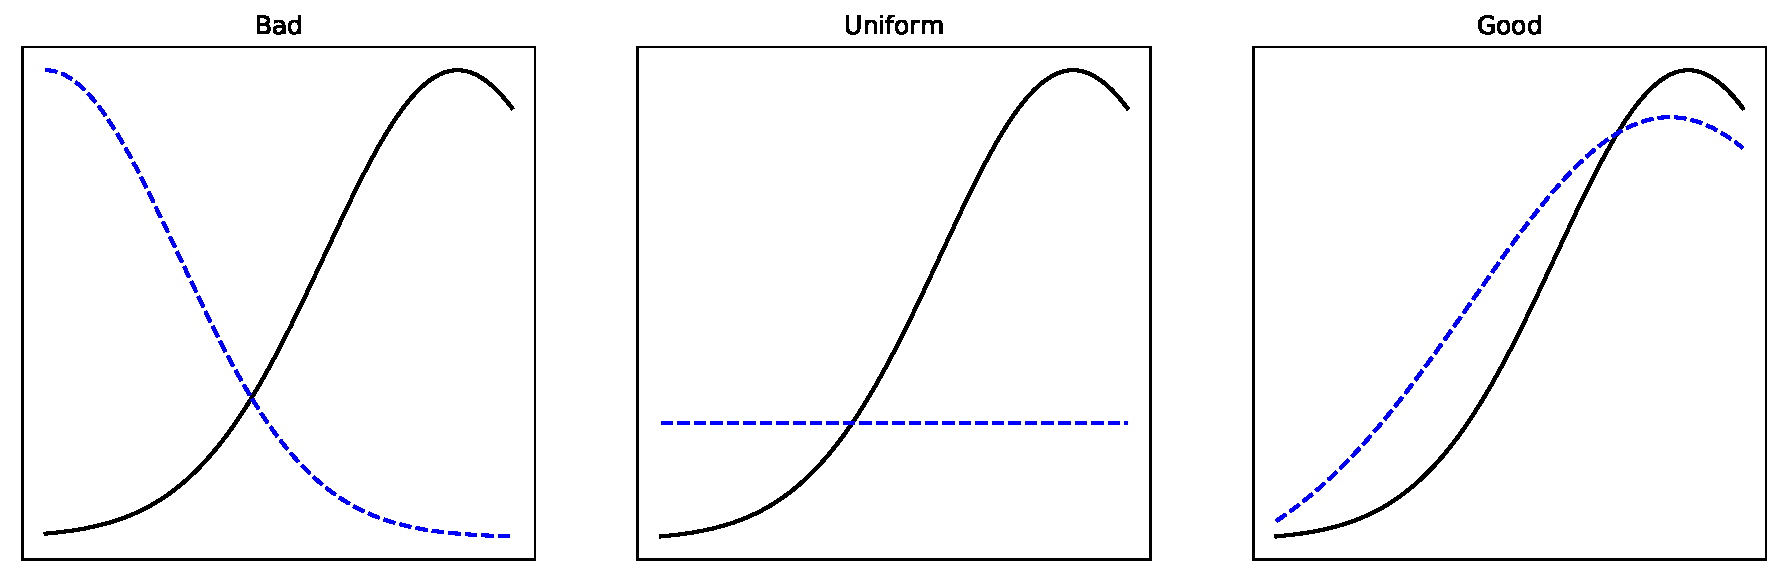
\includegraphics[width=0.8\textwidth]{figures/plots/importancesampling.pdf}
    \caption{.}
    \label{fig:importancesample}
\end{figure}

\subsection{Multiple Importance Sampling}

%% ==============
\section{Bidirectional scattering distribution function}
% mainly only for introduction of specular vs diffuse reflections


%% ==============
\section{Light sources}


%% ==============
\section{Path Tracing}
\subsection{Next Event Estimation}
\label{sec:NEE}


%% ==============
\section{Photon Mapping}
\label{sec:PM}

\subsection{Progressive Photon Mapping}

\subsection{Stochastic Progressive Photon Mapping}



%% ==============
\section{Instant Radiosity}

%% ==============
\section{Datastructures}

% Teapot in a stadium ...

\subsection{Bounding Volume Hierarchy}
\subsection{Grid}
\subsection{Octree}
\subsection{k-d Tree}
\subsection{Surface Area Heuristic}

\section{Interpolation}
\subsection{Scattered data}
\subsection{Structured data}

\label{ch:fu:trilinear}

\begin{figure}
    \centering
    
\includegraphics[width=0.5\textwidth]{figures/img-placeholder.png}
    \caption{The weights are the volume of the opposing rectangle.}
    \label{fig:bilinear}
\end{figure}
\subsection{Global methods}


%% ==============
\section{Machine Learning}

\subsection{Fuzzy k-means}
\subsection{Agglomerative Hierarchical Clustering}
\subsection{Expectation Maximaization}
\subsection{Transductive Support Vector Machine}